% -*- LaTeX -*-
% -*- coding: utf-8 -*-
%
% michael a.g. aïvázis
% california institute of technology
% (c) 1998-2012 all rights reserved
%

\lecture{Three implementations of quadrature rule}{20120206}

% --------------------------------------
% problem statement
\begin{frame}[fragile]
%
  \frametitle{Approximating $\Li$ using a numerical quadrature}
%
  \begin{itemize}
%
  \item the second homework assignment involved $\Li(z)$, defined by
    \begin{equation*}
      \Li(z) \bydef - \int_{0}^{z} dz' \; \frac{\log(1-z')}{z'}
    \end{equation*}
%
    \item the assignment asked for approximating this integral using a simple
      quadrature based on the mid-point rule
      \begin{equation*}
      \Li(z) 
      \approx 
      \Li(z, N) 
      \bydef
      - \frac{z}{N} \sum_{n=0}^{N-1} \left.
        \frac{\log(1-z')}{z'}
      \right|_{z'=(n+\frac{1}{2})\frac{z}{N}}
    \end{equation*}
%
  \end{itemize}
%
\end{frame}

% --------------------------------------
% implementations
\begin{frame}[fragile]
%
  \frametitle{Quadrature rule}
%
  \begin{figure}
    \centering
    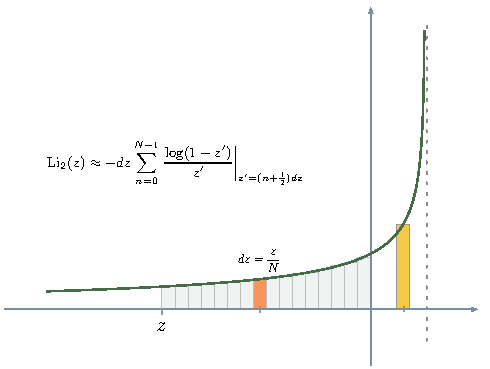
\includegraphics[width=0.9\linewidth]{figures/dilog-quadrature.pdf}
    \label{fig:reduction-shared}
  \end{figure}
%
\end{frame}

%
% --------------------------------------
% implementations
\begin{frame}[fragile]
%
  \frametitle{Implementations}
%
  \begin{itemize}
%
    \item three implementations
      \begin{itemize}
      \item sequential: to get a feeling for how to convert the algorithm into a functioning
        program
      \item parallel using threads: to walk through the parallelization steps and use
        \identifier{pthreads} to get better performance
      \item parallel using \mpi: to get a feel for how \mpi-based programs solve the task
        partitioning problem
      \end{itemize}
%
    \item let's walk through composing, building and running
      \begin{itemize}
      \item on my laptop, and on \href{shc.cacr.caltech.edu}
      \end{itemize}
%
  \end{itemize}
%
\end{frame}

% --------------------------------------
% the sequential driver - preamble
\begin{frame}[fragile]
%
  \frametitle{Sequential implementation - part 1}
%
  \begin{itemize}
  \item the preamble
  \begin{lstlisting}[language=c++,name=sequential]
#include <getopt.h> // for getopt and friends
#include <cstdlib>  // for atof
#include <cmath>    // for the correct abs, log

#include <map>
#include <iostream>
#include <iomanip>
  \end{lstlisting}
%
  \item quadrature using the midpoint rule to avoid the singularities
  \begin{lstlisting}[language=c++,name=sequential]
// dilog
double dilog(double z, long N) {
    // initialize
    double dx = z/N;
    double x = dx/2;
    double sum = 0;
    // loop
    for (long i=0; i < N; i++) {
        sum += std::log(1-x)/x;
        x += dx;
    }
    // return; don't forget the sign
    return -dx * sum;
}

  \end{lstlisting}
%
  \end{itemize}
%
\end{frame}

% --------------------------------------
% the sequential driver - the main program
\begin{frame}[fragile]
%
  \frametitle{Sequential implementation - part 2}
%
  \begin{itemize}
  \item using the command line to set $z$ and the number of subdivisions $N$
  \begin{lstlisting}[language=c++,name=sequential]
// main program
int main(int argc, char* argv[]) {
    //  default values for the command line options
    long N = 1000;
    double z = 1.0;

    // read the command line
    int command;
    while ((command = getopt(argc, argv, "z:N:")) != -1) {
        switch (command) {
        // get the argument of the dilogarithm 
        case 'z':
            z = atof(optarg);
            break;
        // get the number of subdivisions
        case 'N':
            N = (long) atof(optarg);
            break;
        }
    }
  \end{lstlisting}
%
  \end{itemize}
%
\end{frame}

% --------------------------------------
% the sequential driver - the main program
\begin{frame}[fragile]
%
  \frametitle{Sequential implementation - part 3}
%
  \begin{itemize}
  \item error checking and computation of the numerical integral
  \begin{lstlisting}[language=c++,name=sequential]
    // error checking
    // abort if N < 1
    if (N < 1) {
        std::cout 
            << "the number of subdivisions must be positive"
            << std::endl;
        return 0;
    }

    // abort for z > 1 to avoid dealing with the imaginary part
    if (z > 1.0) {
        std::cout << "math domain error: z > 1" << std::endl;
        return 0;
    } 

    // compute
    double value = dilog(z, N);
  \end{lstlisting}
%
  \end{itemize}
%
\end{frame}

% --------------------------------------
% the sequential driver - the main program
\begin{frame}[fragile]
%
  \frametitle{Sequential implementation - part 4}
%
  \begin{itemize}
  \item computing the error and printing out the results
  \begin{lstlisting}[language=c++,name=sequential]
    // build a naive database of the known dilogarithm values
    const double pi = M_PI;
    std::map<double, double> answers;
    answers[1.0] = pi*pi/6;
    answers[-1.0] = -pi*pi/12;

    // print out the value
    std::cout << "Li2(" << z << ")="
        << std::setprecision(17) << std::endl
        << " computed: " << value << std::endl;
    // check whether we know the right answer
    std::map<double,double>::const_iterator lookup = answers.find(z);
    if (lookup != answers.end()) {
        // and if we do, print it out
        double exact = lookup->second;
        std::cout << "    exact: " << exact << std::endl;
        // compute the approximation error and print it out
        double error = std::abs(exact-value)/exact;
        std::cout 
            << std::setiosflags(std::ios_base::scientific) 
            << "    error: " << error << std::endl;
    }

    return 0;
}
  \end{lstlisting}
%
  \end{itemize}
%
\end{frame}

% --------------------------------------
% running the sequential driver
\begin{frame}[fragile]
%
  \frametitle{Building and running the sequential driver}
%
  \begin{shell}{}
#> g++ dilog-quadrature_sequential
#> dilog-sequential -N 1e9 -z 1.0
Li2(1)=
 computed: 1.6449339414016682
    exact: 1.6449340668482264
    error: 7.62623625958871898e-08

real    0m19.885s
user    0m19.877s
sys     0m0.003s
#>
  \end{shell}
%
\end{frame}

% --------------------------------------
% the threaded driver - preamble
\begin{frame}[fragile]
%
  \frametitle{Threaded implementation - part 1}
%
  \begin{itemize}
  \item the preamble
  \begin{lstlisting}[language=c++,name=threaded]
#include <getopt.h> // for getopt and friends
#include <pthread.h>

#include <cstdio>
#include <cstdlib>  // for atof
#include <cmath>

#include <map>
#include <iostream>
#include <iomanip>

  \end{lstlisting}
%
  \end{itemize}
%
\end{frame}

% --------------------------------------
% the threaded driver - thread data structures
\begin{frame}[fragile]
%
  \frametitle{Threaded implementation - part 2}
%
  \begin{itemize}
  \item private and shared data structures
  \begin{lstlisting}[language=c++,name=threaded]
// shared information
struct problem {
    int workers;           // total number of threads
    double dz;             // the width of each subdivision
    double sum;            // storage for the partial computations

    pthread_mutex_t lock;  // mutex to control access to the sum
};

// thread specific information
struct context {
    // thread info
    int id;
    pthread_t descriptor;
    // the workload for this thread
    long subdivisions;  // number of subdivisions
    double z_low;       // the lower limit of integration
    double partial;     // record the partial sum computed by this thread
    // the shared problem information
    problem* info;
};
  \end{lstlisting}
%
  \end{itemize}
%
\end{frame}

% --------------------------------------
% the threaded driver - worker
\begin{frame}[fragile]
%
  \frametitle{Threaded implementation - part 3}
%
  \begin{itemize}
  \item the coarse grain task
  \begin{lstlisting}[language=c++,name=threaded]
// worker
void* worker(void* arg) {
    context* ctxt = (context *) arg;
    // pull the problem information from the thread context
    double dz = ctxt->info->dz;
    double z = ctxt->z_low + dz/2;
    // loop over the subdivisions assigned to this thread
    double sum = 0.0;
    for (long i=0; i < ctxt->subdivisions; i++) {
        sum += std::log(1-z)/z;
        z += dz;
    }
    // multiply by the width of each subdivision and adjust the sign
    sum *= -dz;

    // grab the lock
    pthread_mutex_lock(&(ctxt->info->lock));
    // store the result
    ctxt->info->sum += sum;
    // and release the lock
    pthread_mutex_unlock(&(ctxt->info->lock));

    // all done
    return 0;
}
  \end{lstlisting}
%
  \end{itemize}
%
\end{frame}


% end of file 
